
\documentclass[conference,onecolumn]{IEEEtran}
%\documentclass[article,onecolumn]{IEEEtran}
\usepackage{cite}
\usepackage{amsmath,amssymb,amsfonts}
\usepackage{algorithmic}
\usepackage{graphicx}
\usepackage{textcomp}
\usepackage{xcolor}
\usepackage{float}
\usepackage{subcaption}
\usepackage{multirow}
\usepackage{colortbl}
\usepackage{tabularx}
\usepackage{color}
\usepackage{array}
\usepackage{framed}
\newcolumntype{P}[1]{>{\centering\arraybackslash}p{#1}}
\definecolor{yellow}{rgb}{0.85, 1,1}
\definecolor{pastleyellow}{rgb}{1, 0.98,0.63}
\setlength{\arrayrulewidth}{0.1mm}
\setlength{\tabcolsep}{6pt}
\setlength\headheight{10pt}


\setlength\parskip{1em plus 0.1em minus 0.2em}
\setlength\parindent{0pt}
\setlength{\parskip}{8pt}
\usepackage{subcaption}

\begin{document}

\title{Title\\} %TODO

\author{\IEEEauthorblockN{Authors}\\ %TODO
\IEEEauthorblockA{\textit{Department of Electrical Engineering and Computer Science} \\
\textit{Technische Hochschule Ostwestfalen-Lippe, University of Applied Sciences and Arts}\\
Lemgo, Germany \\
akshay.chikhalkar@stud.th-owl.de, sean.nagel@stud.th-owl.de, kassabji.bassam@stud.th-owl.de}

}

\maketitle
		

\begin{abstract}

\end{abstract}

% Structure of the paper:
% Introduction:
% - IOT Systems lead to many opportunities
% - A case for using IOT can be room management in universities
% - This paper / report discusses a proposed IOT System for room managemt of a university, caled the university Room managemt system
% - The document discusses: Business processes, use cases, user stories to design a domain model and system architecture.
% System description and business process(es)
% Use cases and user stories
% - Short lookout: Use AI tools for specification
% Domain model
% System architecture
% Choosing an appropriate Software development process
% Conclusion/Lookout

\newpage
\tableofcontents

\newpage
\section{Introduction}

\section{Use cases and user stories}

To further identify the desired functionality of the University Room Management System, two use cases and three user stories were identified and formulated.
One use case and two user stories will be described in more detail in this section.

The identified use cases are \emph{Searching and booking a room} and \emph{Getting navigation instructions to a room}.
For the use case \emph{Searching and booking a room} a use case specification was created. The specification is shown in \tablename~\ref{tab:usecasespec}. Some aspects of this use case specification will be further elaborated on.

\begin{table}[tp]
	\centering
	\begin{tabular}{|l|l|}
		\hline
		Name                        & Searching and booking a room \\ \hline
		Scope                       & University Room Management System \\ \hline
		Level                       & User goal \\ \hline
		Primary Actor               & Student, Professor or other university staff \\ \hline
		Stakeholders / interests    & \begin{tabular}[t]{@{}l@{}}Other members of the university (students, professors, other staff)\\ University / university management\end{tabular}\\ \hline
		Preconditions               & User is in possession of a valid university card and has a user account \\ \hline
		Postconditions              & Status of the rooms in the room database is updated \\ \hline
		Main success scenario       & \begin{tabular}[t]{@{}l@{}}
				1. User searches a room via a room number\\
				2. System returns a list of rooms fulfilling the search query\\
				3. User selects a room from the list\\
				4. System shows detailed information about the selected room\\
				5. User books the room\\
				6. System updates booking status of the room\\
				7. System shows booking information and confirmation
			\end{tabular} \\ \hline
		Extensions                  & \begin{tabular}[t]{@{}l@{}}
			1a. User searches room via room properties\\
			\: 1. User opens page to filter specific properties\\
			\: 2. User selects room requirements and confirms\\
			2a. No room fulfilling the search criteria exists\\
			\: 1. System shows message: ``No rooms found''\\
			\: 2. System presents rooms similar to the search query\\
			5a. Room is already booked\\
			\: 1. System shows message: ``Room is already booked''\\
			\: 2. System suggests a list of similar rooms\\
			5b. User already booked the allowed maximum amount of rooms\\
			\: 1. System shows message: ``You cannot book another room''\\
			\: 2. System shows list of rooms already booked by the user\\
			5c. User books room according to a schedule (for future use)\\
			\: 1. System presents a day and time picker\\
			\: 2. User selects day of week and time\\
			\: 3. System asks for the frequency of the booking\\
			\: 4. User selects how often booking should be repeated\\
			\: 5. System books room for all selected time slots\\ 
			\:\: 5a. Room is not available in all time slots\\
			\:\:\: 1. System shows message: ``Room is not available at \textless{}DAY / TIME\textgreater{}''\\
			\:\:\: 2. System provides alternative time slots and rooms\\
			\:\:\: 3. User selects alternatives\end{tabular} \\ \hline
		Special requirements        & \begin{tabular}[t]{@{}l@{}}Stable database\\ Simple UI design\\ Fast search\end{tabular} \\ \hline
		Technology / data variation & Available via a terminal at the university or via a web app \\ \hline
		Frequency of occurrence     & \begin{tabular}[t]{@{}l@{}}Very regularly, up to multiple requests per minute at most active times\\ Long pauses without interaction also likely\end{tabular} \\ \hline
		Open issues                 & Booking of multiple rooms at once \\ \hline
	\end{tabular}
	\caption{Use case specification for the use case \emph{Searching and booking a room}}
	\label{tab:usecasespec}
\end{table}

Extension 1a describes searching for a room via room properties.
Possible properties for searching and filtering rooms could be: type of the room (lecture room or seminar room), room capacity or the availability of projectors and blackboards.

In extension 5b the maximum allowed number of rooms is noted. This limit can be different depending on the user. Our current specification limits students to be allowed of booking only a single room at a given time. University staff is allowed to book multiple rooms at a time (e.g. a Professor booking multiple rooms for an exam). The specific limits for each group of staff should be selected according to the universities specific needs.

Extension 5c notes the possibility to book a room for future use according to a time schedule. This option shall not be available to students but only to university staff. For example a room can be booked for a specific time frame on a weekly basis.
This stands in contrast to the general booking presented in the main success scenario. In that case the room is booked from the time of booking without specifying the length of the booking. The booking has to be terminated manually in the end. Alternatively the booking is also terminated, if the system registers that the room has not been used for a while or a previously scheduled booking is about to start. Please see the BPMN diagram above for this process. %TODO: Link to the figure of the BPMN

The open issues of the use case note the booking of multiple rooms at once.
The process for this will likely be very similar to booking a single room. Showing information for multiple rooms at once and managing the unavailability of a single room ot of the selection need to be further deliberated. Similarly to scheduled booking students should not be allowed to book multiple rooms.

Following three user stories were formulated:

\begin{enumerate}
	\item As a Student, I want to book a room, so that I have a place to work.
	\item As a Guest, I want to have navigational instructions, so that I am able to locate a room.
	\item As a Professor, I want to book a room according to a schedule, so that I can give regular lectures in that room.
\end{enumerate}

A good practice is to formulate user stories according to the INVEST principle.
This principle describes that a user story should be independent, negotiable, valuable, estimable, small and testable.
User stories 1 and 2 were elaborated further and analyzed with regard to the INVEST principle.

The first user story ``As a Student, I want to book a room, so that I have a place to work.'' is extended by following points:

\begin{itemize}
	\item A student is only allowed to book at most one room at any given time.
	\item Students can only book rooms for the current time and are not able to reserve them for later.
	\item A student is identified by their university id.
	\item Bookings by students do not have an ending time specified.
	\item Students are able to terminate their bookings manually.
	\item Bookings by students are terminated automatically, if a booking by a university employee starts.
\end{itemize}

The user story fulfills the INVEST principle, as it does not depend on other user stories, leaves room for negotiation and presents a value to the students.
A development team should be able to estimate the work required for realization. The story itself is small, as it only focuses on bookings for a single user group.
The story can be tested, by students trying to book rooms.

The second user story ``As a Guest, I want to have navigational instructions, so that I am able to locate a room.'' is extended by following points:

\begin{itemize}
	\item The user story is also valid for students and university employees.
	\item Navigation is realized trough  building schematics, as well as indoor and outdoor maps.
	\item Other points of interest (e.g. parking spots, water fountains) are out of scope and might be part of standalone user stories.
	\item Users do not need to be verified for navigation.
\end{itemize}

This user story is independent of other user stories and still leaves room for negotiation. The value of better navigation at the university campus is provided.
The use case is small and the required amount of work can be estimated. Tests might include the navigation between rooms or buildings of the university by external people.
Thus, this use case also fulfills the INVEST principle.

\section{Using machine learning models as specification instruments} \label{sec:chatgpt}

One use case and one user story from the previous section were intentionally not further specified. Instead, they were used to analyze the ability of language models like ChatGPT\footnote{https://openai.com/chatgpt} to generate parts of a system specification.
In particular, we used the aforementioned ChatGPT by OpenAI to generate a use case specification and elaborate on a user story according to the INVEST principle.

The conversation with ChatGPT can be found in appendix~\ref{appdx:chatgpt}.

% About the use case specification

The initial prompt included a short description of the system and asked to write a use case specification for the specific use case.
ChatGPT returned a specification including a name, ID, primary actor, preconditions, postconditions, trigger, main flow, alternate flow, exceptional flow and notes.
To simplify comparisons ChatGPT was asked to provide the specification with the same aspects as those of the specification in \tablename~\ref{tab:usecasespec}.

On first sight, the generated response seems to be good. Some points even include additional explanations. But there are other interesting things to note:

The use case's level was identified as being a user goal and a sub-function. The level should be either one or the other, but not both. by investigating the specification it can be seen, that it should probably be a user goal instead of a sub-function.

The three stakeholders students, professors and guests are identical to the primary actors previously noted in the specification. The only stakeholder, which is not a primary actor is the university management. In this case the primary actors should not be listed in the stakeholders section.

The generated preconditions are relatively simple and are not necessarily needed for the use case specification. Additionally, the third precondition, that the user needs to be logged in, directly contradicts the main success scenario, in which the user is logging in during step 2. Either the precondition or the following scenario is wrong.

The main success scenario starts with the user opening the system application. This is different to our approach, where the scenario started with the application being ready for user interaction. The approach chosen by ChatGPT is not wrong, but just different.
Step 7 and 8 describe how the scenario continues depending on whether a room was found or not. The main success scenario should only contain the successful case of the room being found. The other case should be included as an alternative flow.
Interestingly enough, the single alternative flow of the specification handles this case. Thus, step 8 of the main flow is unnecessary.

For the point frequency of occurrence the generated specification is defined as ``frequently throughout the academic year''. This is a very non-descriptive specification, as it is unclear if the use cases will occur multiple times per hour, per day or per week.

% About the user story

After generating the discussed use case specification ChatGPT was prompted to write a user story using the INVEST principle for user story 3: ``As a Professor, I want to book a room according to a schedule, so that I can give regular lectures in that room.''

The answer starts by listing the six facets of INVEST. It is declared that the given user story fulfills all aspects of the INVEST principle.
Additionally, acceptance criteria for the use case are defined by the language model. The acceptance criteria seem sensible to the use case. Although the first five acceptance criteria are structured very similar to a use cases main success scenario.
The answer also includes some additional considerations, which also seem sensible in the context of the system.

While reading ChatGPT's answer the question arose, how the model would handle a user story, which does not fulfill all aspects of INVEST.
Thus, the model was prompted to write another user story according to the INVEST principle. The user story requested in this prompt is: ``As a University member, I want to use the Room Management System, because it will make life easier.''
This user story is very broad and unspecific, such that it is neither estimable nor small. The user story also is not independent, as it focuses on the entire room management system at once.

The answer of ChatGPT is disappointing, as it is argued that the given user story fulfills all aspects of INVEST. Especially statements like ``The user story has a focused scope'', or ``It focuses on the specific need [...] to utilize the Room Management System'' show that the problems of the user story are not detected by ChatGPT. The task to write the use case done according to the INVEST principle is done, but there is no plausibility check performed.

Although the answers by ChatGPT are not completely correct, the amount of sensible output by the language model are quite impressive, especially if you consider the small amount of information given in the prompts.
The answers of ChatGPT need to be checked for plausibility and cannot be used as is. But the generated use case specifications and user story elaborations can be used as a good starting point, which requires some manual fine-tuning by human designers. Using language models for initial specification drafts can probably decrease the required time for a system specification.

It should also be noted that the used ChatGPT is a general purpose language model. More specified models might yield even better results.
Currently, there are developments on models with the specific task to generate such specification and even write some initial code. One example that should be noted in this context is ``MetaGPT''\footnote{https://github.com/geekan/MetaGPT}, which according to its development page is able to generate user stories, requirements, APIs and more.




%%%%%%%% Domain Model (Akshay)%%%%%%%%%
\section{Domain model}
The domain model is visual representation of real objects and conceptual classes. 

\subsection{Conceptual classes}
	The conceptual classes for the University Room Management System (URMS) are shown in \tablename~\ref{tab:conceptualclasses} below.

	\begin{table}[h]
		\centering
		\begin{tabular}{|l|l|}
			\hline
			Business transactions                       & Booking (includes reservations implicitly) \\ \hline
			Transaction line items                      & Booking time frame \\ \hline
			Product/service                       		& \begin{tabular}[t]{@{}l@{}}
																Room \\
																Navigation Instructions
															\end{tabular} \\ \hline
			Transaction record               			& - \\ \hline
			Actors									    & \begin{tabular}[t]{@{}l@{}}
																Students \\ 
																Guests \\
																Professors \\
																Other university employees
															\end{tabular} \\ \hline
			Place               					 	& \begin{tabular}[t]{@{}l@{}}
																University campus \\ 
																Software Frontend (System user interface)
															\end{tabular} \\ \hline
			Events              						& Bookings \\ \hline
			Physical objects       						& \begin{tabular}[t]{@{}l@{}}
																Rooms \\
																Buildings \\
																Room display \\
																Door lock \\
																Movement sensor
															\end{tabular} \\ \hline
			Descriptions                  				& - \\ \hline
			Catalouge        							& - \\ \hline
			Container									& \begin{tabular}[t]{@{}l@{}}
																Room \\ 
																Building \\
																Campus
															\end{tabular} \\ \hline
			Things in container						    & \begin{tabular}[t]{@{}l@{}}
																Building \\ 
																Room \\
																Room display \\
																Door lock \\
																Movement sensor
															\end{tabular} \\ \hline
			Neighboring systems                 		& - \\ \hline
			Records                 					& Booking \\ \hline
			Financial instruments                 		& - \\ \hline
			Schedules/manuals                 			& Room schedule \\ \hline

		\end{tabular}
		\caption{Conceptual classes for the University Room Management System}
		\label{tab:conceptualclasses}
	\end{table}

	%%%%%% Need to review %%%% @akshay
	% In the context of a use case ``Searching and Booking a Room'', several conceptual classes are identified to categorise and describe various aspects of the system. Business transactions, represented by actions like ``Booking'', encapsulate user interactions involving reserving a room, implicitly including reservations. Transaction line items, such as ``Booking time frame'', delineate specific details within these transactions, like the duration of the booking. Products or services, exemplified by ``Room'' and ``Navigation Instructions'', signify offerings available for interaction within the system, with rooms being bookable entities and navigation instructions aiding users. Actors, encompassing ``Students'', ``Guests'', ``Professors'', and ``Other university employees'', denote distinct user roles interacting with the system. ``Place'' conceptualises both tangible and virtual locations like the ``University campus'' and the ``Software Frontend'', the latter being the user interface. ``Events'', in this case, ``Bookings'', denote significant occurrences within the system. Physical objects, such as ``Rooms'', ``Buildings'', ``Room display'', ``Door lock'', and ``Movement sensor'', represent tangible entities within the environment. Containers, including ``Room'', ``Building'', and ``Campus'', group entities within larger contexts. ``Things in container'', consisting of items like ``Building'', ``Room'', ``Room display'', ``Door lock'', and ``Movement sensor'', describe components held within these containers. While ``Descriptions'' and ``Catalogue'' are mentioned without specific instances, ``Neighbouring systems'' indicates interactions with external systems. ``Records'', exemplified by ``Booking'', signify formal recordings of user actions. The concept of ``Financial instruments'' refers to unspecified financial tools, and ``Schedules/manuals'', like ``Room schedule'', represent plans or guides outlining specific system aspects.

	The conceptual classes helps to clarify how different elements interact within the system. These conceptual classes provide a way to categorize the key aspects of the system. The system's ``business transactions'' involve actions like making room reservations or bookings. Each transaction is further detailed through ``transaction line items,'' which specify aspects such as the timeframe for a room reservation. The ``product/service'' category encompasses items like rooms and navigation instructions, while ``actors'' refers to the different individuals who interact with the system, such as students, professors, guests, and university staff.
	
	``Place'' pertains to relevant locations, including the university campus and the user interface of the system itself. Events like bookings are tracked under ``events,'' while ``physical objects'' encompass tangible items like rooms, buildings, and sensors.
	
	``Container'' refers to broader categories like buildings, rooms, and the campus, while ``things in container'' delves into specific instances within those categories, such as individual rooms and door locks. The concept of ``neighboring systems'' highlights potential interactions with other external systems.
	
	``Records'' represent the detailed information about bookings made within the system. ``Schedules/manuals'' involve information related to room schedules or guidelines. These conceptual classes help paint a comprehensive picture of how the University Room Management System operates and how its various components fit together.

\subsection{Class diagram}
	The class diagram illustrates the structure and relationship among classes in the system. The university room management system includes total of 13 classes which are shown in \figurename~\ref{fig:classdiagram} below.

	\begin{figure}[H]
		\centering
		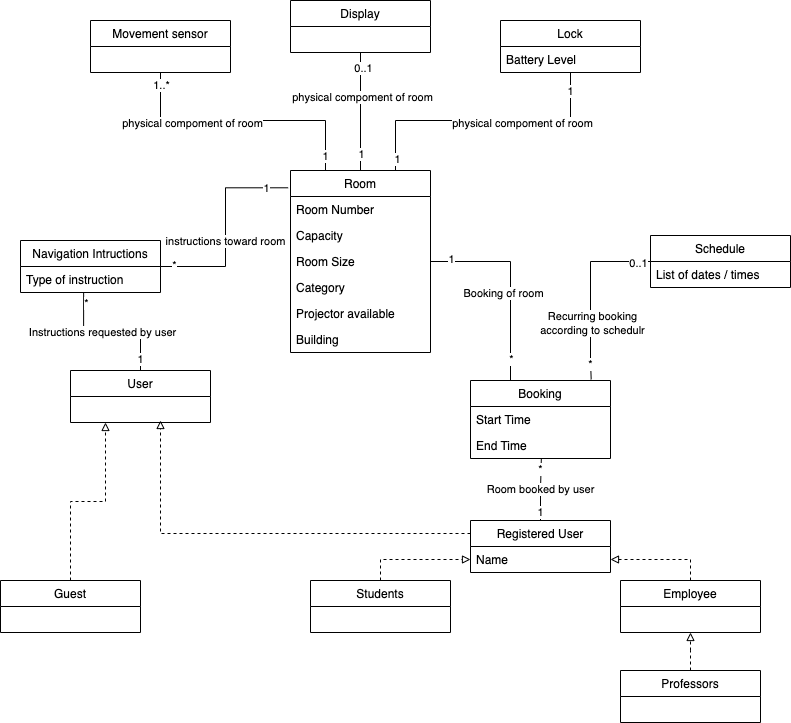
\includegraphics[width=0.6\textwidth]{Images/DomainModel.png}
		\caption{Domain model of the University Room Management System}
		\label{fig:classdiagram}
	\end{figure}

	\subsubsection*{Classes}
		The classes is an amalgamation of physical objects and software components. The classes are described below:
		Movement sensor: The movement sensor is a physical object which is used to detect the presence of a person in the room. It is connected to the room display and the door lock through the system (Room). At least one movement sensor is present in each room and connected to the class ``Room'' in many-to-one association, refer to \figurename~\ref{fig:classdiagram}.
		
		Display: The display is a physical object which displays the room schedule and other booking information. In this system we consider no or more that one display per room and connected to the class ``Room'' in one-to-many association, refer to \figurename~\ref{fig:classdiagram}.

		Lock: The lock is again a physical object which is used to lock and unlock the room. In this system we consider one lock per room and connected to the class ``Room'' in one-to-one association, refer to \figurename~\ref{fig:classdiagram}. The class ``Lock'' has one attribute ``Battery Level'' which is used to check the status of the Battery and helps to keep track of maintenance cycles.

		Navigation Instructions: The navigation instructions is a service which is used to provide directions or visual insight to the user. Navigation instructions can be invoked by the system itself or by the user. This can be achieved by requesting navigation instructions at the time of booking or by accessing navigation service and search for the room number. The class ``Navigation Instructions'' has one attribute ``Type of instruction'' which defines whether instructions are requested in the building schematics or maps form. It is associated with the class ``Room'' and ``User'' in many-to-one association, refer to \figurename~\ref{fig:classdiagram}.

		Schedule: The class ``Schedule'' holds the schedule metadata about the lectures according to scheduler. This schedule can be referred by the user at the time of booking to create recurring room reservations. The attribute ``List of dates / times'' returns the all the days and time of the week when the lecture is scheduled. The class ``Schedule'' is associated with the class ``Booking'' in one-to-many (0...1 to *) association, refer to \figurename~\ref{fig:classdiagram}.

		Booking: The class ``Booking'' holds the booking metadata about the room reservations. The attributes ``Start Time'' and ``End Time'' returns the start and end time of the booking. It invokes class ``Schedule'' to get lecture schedule if required. The class ``Booking'' is associated with the class ``Room'', ``Schedule'' and ``Registered User'' in many-to-one association, refer to \figurename~\ref{fig:classdiagram}.

		Registered User: The class ``Registered User'' is master class for university students, professors and other university staff. It means, these users are authenticated via valid student or employee ID. The classes ``Student'', ``Professors'' and ``Employee'' are inherited from the class ``Registered User'' and associated with the class ``Booking'' in one-to-many (1 to *) association, refer to \figurename~\ref{fig:classdiagram}.

		Guest: The class ``Guest'' is a user who is not registered in the system. It is inherited from the class ``User'' and has limited privileges in the system such as requesting navigational instructions.

		User: The class ``User'' is a master class for all the users in the system. It is associated with the class ``Navigation Instructions'' in one-to-many (1 to *) association, refer to \figurename~\ref{fig:classdiagram}.

		Room: The class ``Room'' is a software component which is used to represent the physical room. It is associated with the classes ``Booking'', ``Navigation Instructions'', ``Display'', ``Lock'' (1 to 1), ``Movement Sensor'' and ``Booking'' in one-to-many (1 to *) association, refer to \figurename~\ref{fig:classdiagram}. ``Room'' contains total of 6 attributes which are described below:
		``Room Number'': The attribute ``Room Number'' is used to identify the room uniquely. It is a primary key for the class ``Room''.
		``Capacity'': The attribute ``Room Capacity'' is used to identify the capacity of the room or number of people it can fit.
		``Room Size'': The attribute ``Room Size'' is used to identify the size of the room in square meters.
		``Category'': The attribute ``Category'' is used to identify the type of the room such as lecture room, seminar room, etc.
		``Projector available'': The attribute ``Projector available'' is used to identify whether the room has projector or not.
		``Building'': The attribute ``Building'' is used to identify the building in which the room is located.


%%%%%%%% System Architecture (Akshay)%%%%%%%%%
%\section{System architecture}




\section{Experiment and Results}
\section{Discussion}


\section{Conclusion}

% use section* for acknowledgment
\section*{Acknowledgment}

\newpage
%\section*{Appendix}
\appendix

\subsection{Conversation with ChatGPT} \label{appdx:chatgpt}
 
The conversation with ChatGPT described in section~\ref{sec:chatgpt}:

Prompt:
\begin{framed}
	\small
	A University Manager system, which is a system where students can book lecture rooms at the university for study and professors can book seminar rooms to give lectures. In addition the University Manager system, give the possibility for students, professor and guests  to have navigation instruction for a seminar room they search for.
	
	Write me a use-case specification using the proper and formal structure for that.
	
	A use case specification for the use case called (getting navigation instructions to a seminar room in the university) that is implemented in the University Manager system.
\end{framed}

Answer:
\begin{framed}
	\small
	\textbf{Use Case Specification: Getting Navigation Instructions to a Seminar Room in the University}
	
	\textbf{Use Case Name:} Get Navigation Instructions to a Seminar Room
	
	\textbf{ID:} UC-NAV-01
	
	\textbf{Description:} This use case allows students, professors, and guests using the University Manager system to obtain navigation instructions to reach a specific seminar room within the university campus. Users can search for a seminar room by its room number or name, and the system will provide step-by-step directions to help them reach the desired location.
	
	\textbf{Primary Actor:} User (Student, Professor, or Guest)
	
	\textbf{Preconditions:}
	
	\begin{itemize}
		\item The University Manager system is up and running.
		\item The user is logged into the system (for registered students and professors).
	\end{itemize}
	
	\textbf{Postconditions:}
	
	\begin{itemize}
		\item The user receives navigation instructions to the requested seminar room.
	\end{itemize}
	
	\textbf{Trigger:} User initiates the request to get navigation instructions to a seminar room.
	
	\textbf{Main Flow:}
	
	\begin{enumerate}
		\item     The user opens the University Manager system's application or website.
		\item If required, the user logs into the system using their credentials. (Skipped for guests)
		\item The user selects the option to "Get Navigation Instructions" from the main menu.
		\item The system presents the user with a search bar to enter the seminar room number or name they wish to navigate to.
		\item The user enters the seminar room number or name in the search bar.
		\item The system validates the entered information and searches for the requested seminar room in the database.
		\item If the seminar room is found:\\
		a. The system calculates the best route to reach the seminar room from the user's current location or a specified starting point within the campus.\\
		b. The system generates step-by-step navigation instructions, including directional cues (e.g., left, right, straight), landmarks, and approximate distances.\\
		c. The navigation instructions are displayed on the user's device screen.
		\item If the seminar room is not found:\\
		a. The system displays an error message indicating that the seminar room could not be located.\\
		b. The use case terminates.
	\end{enumerate}
	
	\textbf{Alternate Flow:}
	
	6a. If the entered seminar room number or name is not valid or does not exist:\\
	i. The system displays an error message indicating that the seminar room could not be found.\\
	ii. The user is given the option to re-enter the room number or name.\\
	iii. The user may choose to cancel the navigation request.\\
	iv. The use case continues from step 4.
	
	\textbf{Exceptional Flow:}
	
	\begin{enumerate}
		\item If the University Manager system is not operational due to maintenance or technical issues:\\
		a. The user is informed about the unavailability of the system.\\
		b. The user may be asked to try again later or contact support for assistance.\\
		c. The use case terminates.
	\end{enumerate}
	
	\textbf{Notes:}
	
	\begin{itemize}
		\item The University Manager system may integrate with campus maps or GPS services to provide accurate navigation instructions.
		\item The system could offer additional features, such as displaying accessibility information or estimated time of arrival to the seminar room.
		\item For security reasons, certain seminar rooms (e.g., faculty offices) may have restricted access for navigation instructions. In such cases, the system should inform the user accordingly.
	\end{itemize}
\end{framed}

Prompt:
\begin{framed}
	\small
	Use Case Specification: Getting Navigation Instructions to a Seminar Room in the University in terms of :\\
	Name\\
	Scope\\
	Level\\
	Primary actor \\
	Stakeholders\\
	preconditions\\
	postconditions\\
	Main success scenario\\
	Extensions\\
	Special requirements:\\
	Technology / data variation: \\
	Frequency of occurence: \\
	Open issues:
\end{framed}

Answer:
\begin{framed}
	\small
	\textbf{Name:} Getting Navigation Instructions to a Seminar Room in the University
	
	\textbf{Scope:} University Manager System
	
	\textbf{Level:} User Goal (Primary), Subfunction (Secondary)
	
	\textbf{Primary Actor:} User (Student, Professor, or Guest)
	
	\textbf{Stakeholders:}
	
	\begin{itemize}
		\item Students: Require navigation instructions to find seminar rooms for academic purposes.
		\item Professors: Need navigation guidance to reach seminar rooms for conducting lectures or meetings.
		\item Guests: Visitors to the university who may require navigation assistance to attend seminars or events.
		\item University Management: Ensures the system enhances campus navigation and user experience.
	\end{itemize}
	
	\textbf{Preconditions:}
	
	\begin{itemize}
		\item The University Manager system is operational and accessible to the primary actor.
		\item The user has a compatible device with access to the University Manager system.
		\item For registered students and professors, the user is logged into the system.
	\end{itemize}
	
	\textbf{Postconditions:}
	
	\begin{itemize}
		\item The user receives accurate navigation instructions to the requested seminar room within the university campus.
	\end{itemize}
	
	\textbf{Main Success Scenario:}
	
	\begin{enumerate}
		\item The user opens the University Manager system's application or website.
		\item If required, the user logs into the system using their credentials. (Skipped for guests)
		\item The user selects the option to "Get Navigation Instructions" from the main menu.
		\item The system presents the user with a search bar to enter the seminar room number or name they wish to navigate to.
		\item The user enters the seminar room number or name in the search bar.
		\item The system validates the entered information and searches for the requested seminar room in the database.
		\item If the seminar room is found:\\
		a. The system calculates the best route to reach the seminar room from the user's current location or a specified starting point within the campus.\\
		b. The system generates step-by-step navigation instructions, including directional cues (e.g., left, right, straight), landmarks, and approximate distances.
		c. The navigation instructions are displayed on the user's device screen.
		\item If the seminar room is not found:\\
		a. The system displays an error message indicating that the seminar room could not be located.\\
		b. The user is given the option to re-enter the room number or name.\\
		c. The user may choose to cancel the navigation request.
	\end{enumerate}
	
	\textbf{Extensions:}
	
	6a. If the entered seminar room number or name is not valid or does not exist:\\
	i. The system displays an error message indicating that the seminar room could not be found.\\
	ii. The user is prompted to re-enter the room number or name.\\
	iii. The user may choose to cancel the navigation request.\\
	iv. The use case continues from step 4.
	
	\textbf{Special Requirements:}
	
	\begin{itemize}
		\item The University Manager system should integrate with campus maps or GPS services for accurate navigation.
		\item The system may provide additional features such as displaying accessibility information or estimated time of arrival to the seminar room.
		\item Certain seminar rooms may have restricted access, and the system should handle these cases appropriately.
	\end{itemize}
	
	\textbf{Technology / Data Variation:}
	
	\begin{itemize}
		\item The system should be accessible via various platforms (web, mobile apps) to accommodate different user devices.
		\item The availability of campus map data and GPS accuracy may vary depending on the university's infrastructure.
	\end{itemize}
	
	\textbf{Frequency of Occurrence:}
	
	\begin{itemize}
		\item The use case is expected to occur frequently throughout the academic year as students attend lectures, professors conduct classes, and events are held.
	\end{itemize}
	
	\textbf{Open Issues:}
	
	\begin{itemize}
		\item How will the system handle navigation to seminar rooms located in different buildings or floors within the campus?
		\item Should the system provide additional options such as displaying alternative routes or real-time updates for room availability?
		\item How will the system ensure privacy and security of users' location data while providing navigation instructions?
	\end{itemize}
\end{framed}

Prompt:
\begin{framed}
	\small
	write me a user story using the INVEST principal for the following user story:
	
	user story: As a Professor, I want to book a room according to a schedule so that I can give regular lectures in that room.
\end{framed}

Answer:
\begin{framed}
	\small
	\textbf{User Story:} As a Professor, I want to book a room according to a schedule so that I can give regular lectures in that room.
	
	\textbf{INVEST Principle:}
	
	\begin{itemize}
		\item \textbf{Independent:} The user story is self-contained and can be implemented without dependencies on other user stories. It focuses on the specific need of the Professor to book a room for regular lectures.
		
		\item \textbf{Negotiable:} The details of the implementation are open to negotiation between the Professor (user) and the development team. The team can collaborate with the Professor to determine the specific room booking requirements and scheduling preferences.
		
		\item \textbf{Valuable:} The user story provides clear value to the Professor by enabling them to secure a designated room for their regular lectures, ensuring consistent teaching arrangements and an organized learning environment.
		
		\item \textbf{Estimable:} The user story is well-defined and has a clear scope, making it estimable for the development team. The effort required to implement the room booking functionality can be reasonably assessed.
		
		\item \textbf{Small:} The user story has a focused and concise scope, which allows the development team to implement it within a single development iteration.
		
		\item \textbf{Testable:} The user story's acceptance criteria are specific and measurable, allowing for effective testing. It is possible to verify the successful implementation of the room booking feature based on the defined criteria.
	\end{itemize}
	
	\textbf{Acceptance Criteria:}
	
	\begin{itemize}
		\item The Professor can access the University Manager system and navigate to the "Room Booking" section.
		\item The system presents a form with options to select the desired room, date, start time, and end time for the lecture.
		\item The Professor can enter the required details and submit the booking request.
		\item The system validates the availability of the selected room for the specified date and time.
		\item If the room is available, the system confirms the booking and sends a confirmation email to the Professor.
		\item The booked room should be reserved in the system's schedule for the specified date and time.
		\item The Professor can view, modify, or cancel their booked lectures within the system as needed.
		\item In case of any conflicts or unavailability, the system provides alternative room options or available time slots for the Professor's lectures.
		\item The system ensures that only authorized Professors can access the room booking functionality.
	\end{itemize}
	
	\textbf{Additional Considerations:}
	
	\begin{itemize}
		\item The system should have user authentication to ensure that only authorized Professors can access the room booking feature.
		\item The system may send reminders or notifications to the Professor before the scheduled lecture time.
		\item The room booking feature should be user-friendly and accessible via multiple platforms, such as web and mobile applications.
		\item The system should handle and display room availability in real-time to avoid double bookings.
		\item The user interface should be intuitive and provide clear feedback on the status of the room booking process.
	\end{itemize}
	
	Note: The user story may be further elaborated during backlog grooming or refinement sessions to capture more detailed requirements and user expectations.
\end{framed}

Prompt:
\begin{framed}
	\small
	write me a user story using the INVEST principal for the following user story:
	
	user story: 
	As a University member, I want to use the Room Management System, because it will make life easier.
\end{framed}

Answer:
\begin{framed}
	\small
	\textbf{User Story:} As a University member, I want to use the Room Management System because it will make life easier.
	
	\textbf{INVEST Principle:}
	
	\begin{itemize}
		\item \textbf{Independent:} The user story is self-contained and can be implemented independently without relying on other user stories. It focuses on the specific need of the University member to utilize the Room Management System for simplifying room-related tasks.
		
		\item \textbf{Negotiable:} The user story allows for negotiation between the University member (user) and the development team to identify the specific features and functionalities that will enhance their experience with the Room Management System.
		
		\item \textbf{Valuable:} The user story holds clear value for the University member by offering a convenient and efficient solution for managing room-related activities, streamlining processes, and saving time.
		
		\item \textbf{Estimable:} The user story is well-defined and has a clear scope, making it estimable for the development team. The effort required to implement the Room Management System features can be reasonably estimated.
		
		\item \textbf{Small:} The user story has a focused scope, enabling the development team to implement it within a single development iteration.
		
		\item \textbf{Testable:} The user story's acceptance criteria are specific and measurable, enabling effective testing. The success of the Room Management System can be assessed based on the defined criteria.
	\end{itemize}
	
	\textbf{Acceptance Criteria:}
	
	\begin{itemize}
		\item The Room Management System should be accessible to all University members through a user-friendly web application or mobile interface.
		\item The system should have user authentication to ensure that only authorized University members can access and use the Room Management features.
		\item University members should be able to log in using their credentials or university ID.
		\item The Room Management System should provide a clear and intuitive user interface with navigational menus and visual cues.
		\item University members should be able to view available rooms, their schedules, and occupancy status in real-time.
		\item The system should offer a simple and efficient process for booking or reserving rooms for various purposes (e.g., lectures, study sessions, meetings).
		\item Room availability should be displayed in a visual calendar format, with filtering options based on date, time, location, or room amenities.
		\item The system should send notifications or reminders to users about upcoming room reservations or changes in room status.
		\item University members should be able to easily modify or cancel their room reservations within the system.
		\item The Room Management System should maintain accurate and up-to-date records of room bookings and usage.
		\item The system should have a responsive design to ensure usability across different devices and screen sizes.
	\end{itemize}
	
	\textbf{Additional Considerations:}
	
	\begin{itemize}
		\item The Room Management System could incorporate features like room occupancy limits, equipment availability, and room-specific details.
		\item To enhance user adoption, the system could provide user tutorials or help documentation for first-time users.
		\item The system should prioritize data security and privacy, ensuring that only authorized personnel can access sensitive room-related information.
		\item Regular user feedback and iterative improvements can be incorporated to enhance the Room Management System based on user preferences and needs.
	\end{itemize}
	
	Note: The user story may be further elaborated during backlog grooming or refinement sessions to capture more detailed requirements and user expectations
\end{framed}
 
\newpage
\bibliographystyle{IEEEtran}
\bibliography{ref}
\end{document}